%% ceci est un commentaire 
%% il faut toujours commencer par \documentclass[type de papier, taille de texte]{sytle du document}
\documentclass[a4paper,10pt]{report} %%%% sytle du document : report/book/article


%%%%%%%%%%%%%%%%%%%%%%%%%%%%%%%%%%%%%%%%%%%%%%%%%%%%%%%%%%%%%%%%%%%%%%%%%%%%%%%
%% la suite est une collection des "package" ou des "librararies" pour utiliser des codes spécifiques

%% il vous suffit de les copie-coller quand vous créez un nouveau document TeX (ou bien en ajouter plus si besoin).
\usepackage[utf8]{inputenc} %% pour les accents en français
\usepackage[frenchb]{babel} %% pour un format français
\usepackage{graphicx} %% pour afficher des graphiques
\usepackage{amsmath} %% pour écrire des symboles (maths), des équations, etc.
\usepackage{float}
\usepackage{amssymb}
\usepackage{color}
\usepackage{bm} %% pour lister des citations/la biblio
\usepackage{hyperref} %% pour inserer des liens internet
%\usepackage{cleveref} %% pour faire des références uax équations, tableaux, etc.
%\usepackage{setspace} %% pour changer l'espace entre les lignes
%\linespread{1.6} %% pour changer l'espace entre les lignes












%%%%%%%%%%%%%%%%%%%%%%%%%%%%%%%%%%%%%%%%%%%%%%%%%%%%%%%%%%%%%%%%%%%%%%%%%%%%%%%
\title{--------\textbf{Turbinee Pelton}--------} %% choissez un titre approprié à votre sujet
\author{par\\ZHANG Xunjie \\ pour Turbomachines TP M1} %% utilisez \\ pour une novuelle ligne
\date{fait le 25 mai 2017} %% pour afficher la date actuelle commenter cette ligne








%%%%%%%%%%%%%%%%%%%%%%%%%%%%%%%%%%%%%%%%%%%%%%%%%%%%%%%%%%%%%%%%%%%%%%%%%%%%%%%
%% TOUT ce qui va dans votre rapport doit être entre \begin{document} & \end{document}
\begin{document}
\selectlanguage{french} %% format français
\maketitle %% pour afficher le titre
%\tableofcontents %% pour afficher/compiler le sommaire automatiquement
%\listoffigures %% pour lister les figures






%%%%%%%%%%%%%%%%%%%%%%%%%%%%%%%%%%%%%%%%%%%%%%%%%%%%%%%%%%%%%%%%%%%%%%%%%%%%%%%
\chapter{Introduction} %% pour commencer un chapitre





%%%%%%%%%%%%%%%%%%%%%%%%%%%%%%%%%%%%%%%%%%%%%%%%%%%%%%%%%%%%%%%%%%%%%%%%%%%%%%%
\section{Introduction} %% pour commencer une section

\begin{figure}[h!]
\centering
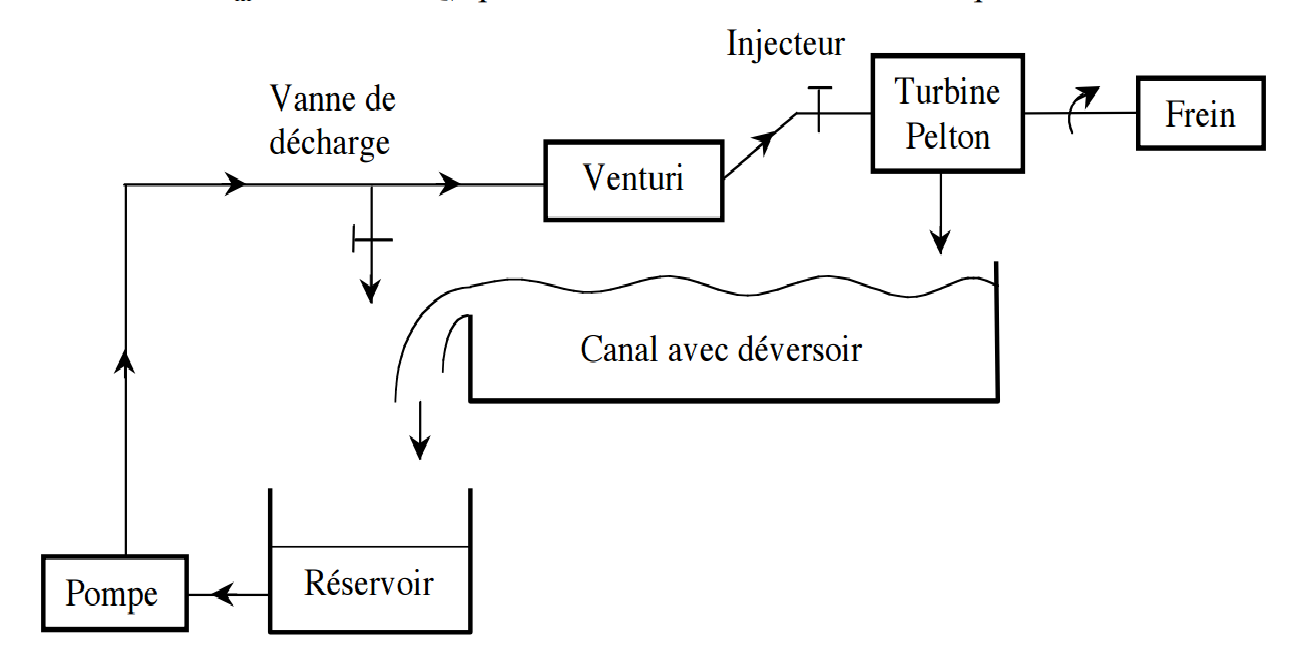
\includegraphics[width=1.0\textwidth]{fig/figure1.png}
\caption{equipement}
\end{figure}

L'utilisation des turbines hydrauliques a pour principal objectif de récupérer l'énergie cinétique du fluide après une chute d'une certaine hauteur.L'arbre de la machine hydraulique récupère l'énergie sous forme de puissance. Dans notre cas, on va qu'une turbine Pelton fait une simulation d'une chute d'eau en utilisant un certain débit de fluide.\\

L'eau est envoyée sous pression dans le plan de la roue par une pompe à l'entrée de la turbine, simulant ainsi une certaine hauteur de chute.\\

Lors de ce TP, on a pris deux valeurs d'étude pour la hauteur de chute $Hm_1=23$ mètre de colonnes d'eau et $Hm_2=29$ mètres de colonnes d'eau.\\

Les turbines Pelton sont des turbines à action, c'est à dire que seule l'énergie cinétique du fluide est récupérée par l'arbre sous forme de puissance.\\



\section{Problème physique}
\begin{figure}[h!]
\centering
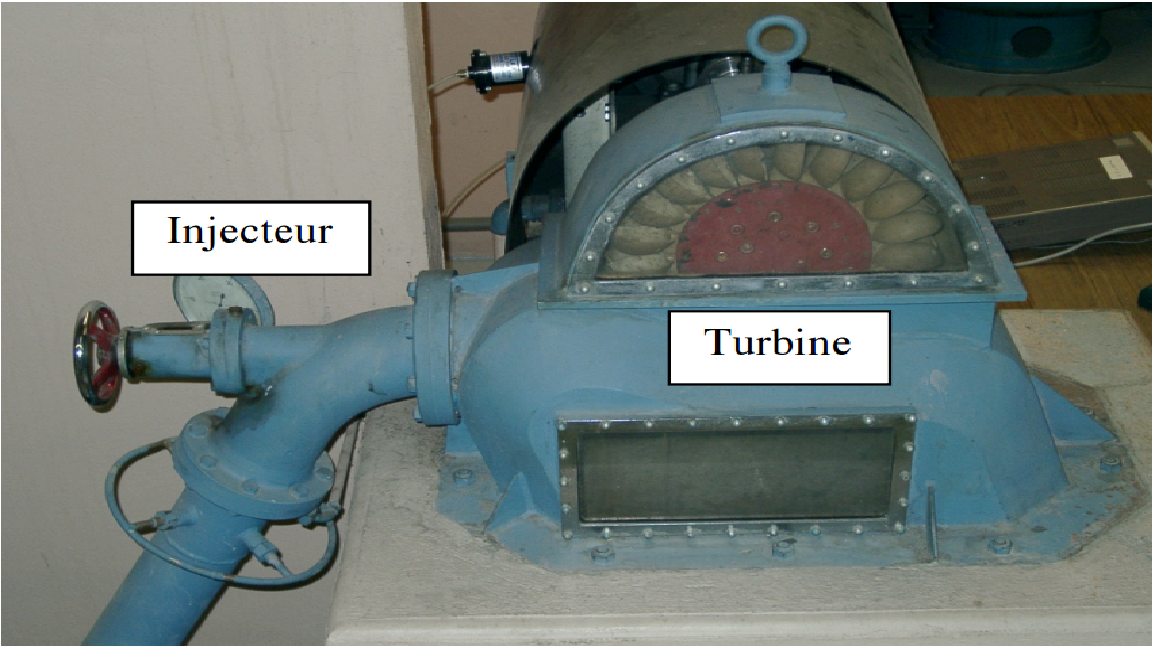
\includegraphics[width=1.0\textwidth]{fig/figure2.png}
\caption{equipement reel}
\end{figure}

Pour simplifier le problème, nous faisons différentes hypothèses concernant le fluide et l'écoulement.


\begin{figure}[h!]
\centering
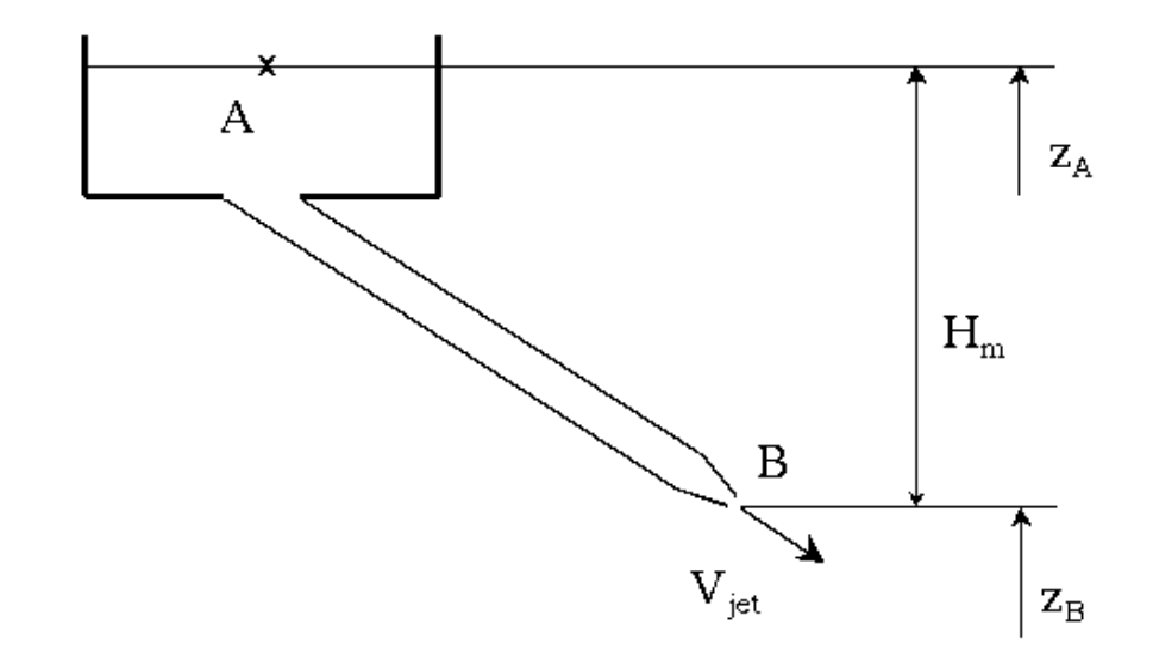
\includegraphics[width=1.0\textwidth]{fig/figure3.png}
\caption{etat équivalent}
\end{figure}

On commence par se placer sur un modèle incompressible avec $\rho(p,T)=cte$.

On utilise ensuite la loi Hydrostatique qui nous donne :

$$P_0-P_{atm}=\rho g H_m$$
$$H_m=\frac{P_0-P_{atm}}{\rho g}$$

Avec l'utilisation du théorème de Bernoulli pour un fluide incompressible, stationnaire et non-visqueux : 




$$p+\frac{\rho V^2}{2}+\rho g z=cte$$

$$p_0+\frac{1}{2} \rho V_0^2=p_{atm} + \frac{1}{2} \rho V_j^2$$

On fait l'hypothèse que la vitesse au point A est négligeable , on obtient :

$$\frac{1}{2} \rho V_j^2=p_0-p_{atm}=\rho g H_m$$

et donc la puissance disponible dans le jet est :

$$\frac{1}{2} \rho V_j^2 * \frac{V}{\Delta t}$$

Avec $\frac{\rho V_j^2}{2}$ Une énergie cinétique par unité de volume et $\frac{V}{\Delta t}$


Pour caractériser le comportement de la machine hydraulique, on construit les coefficients adimensionnels (de Rateau) et on déduit un nombre de variables indépendantes qui décrivent la physique du problème :

\begin{itemize}
\item D le diamètre en mètres.
\item La viscosité dynamique $\mu$ du fluide.
\item La masse volumique $\rho$ du fluide.
\item La hauteur de chute $H_m$.
\item La vitesse de rotation $N$ de l'arbre.
\item Le débit $Q_v$ en fonction de la position de l'injecteur.
\end{itemize}

Pour 6 variables indépendantes et 3 unités ($M,L,T$), on déduit les groupements adimensionnels :

$$M_1=\frac{Q_v}{D^2 \sqrt{g H_m}}$$

$$M_2=\frac{\mu}{\rho D \sqrt{g H_m}}$$

$$M_3=\frac{N D}{\sqrt{g H_m}}$$

$$N_{11}=\frac{N D }{\sqrt{g H_m}}$$

$$C_{11}=\frac{C}{\rho g H_m D^3}$$ 

$$W_{11}=\frac{C N}{\rho D^2 (g H_m)^{\frac{3}{2}}}$$

On a aussi le rendement défini comme le rapport de la puissance récupérée et de la puissance disponible :

$$\eta=\frac{C N}{\rho g H_m}$$

\chapter{Etude Expérience} 

Dans cette partie, nous allons calculer la valeur du débit à l'aide d'un tube de Venturi:\\
Nous avons pour cela prélevé deux hauteurs pour $H_{m1},H_{m2}$\\
Pour $H_{m1}$: h=166mm,
On utilise ensuite la loi Hydrostatique qui nous donne :

$$P_{0}-P_{atm}=\rho*g H_m$$

$$H_m=\frac{P_0-P_{atm}}{\rho g}$$
D'après la formule fournie dans la fiche technique on a :\\
$\Delta{P}=(\rho_{mercure}-\rho_{eau})g *\Delta{h}$\\
Avec $$\rho_{mercure}=13546 kg/m^3$$
$$\rho_{eau}=1000 kg/m^3$$
$\Delta{P}=2.04 Pa$.\\

D'après la formule donnée sur la fiche technique:\\
$Q_{v}(m^{3}/s)=0.00915*\sqrt{\Delta{P}}=0.013$


Pour $H_{m2}$: $h=121mm$,
On utilise ensuite la loi Hydrostatique qui nous donne :

$$P_{0}-P_{atm}=\rho*g H_m$$
$$H_m=\frac{P_0-P_{atm}}{\rho g}$$
D'après la formule fournie dans la fiche technique on a :\\
$\Delta{P}=(\rho_{mercure}-\rho_{eau})g *\Delta{h}$\\
Avec $$\rho_{mercure}=13546 kg/m^3$$
$$\rho_{eau}=1000 kg/m^3$$
$$\Delta{P}=1.49 Pa$$
Donc,$Q_{v}(m^{3}/s)=0.00915*\sqrt{\Delta{P}}=0.01117$.\\

Maintenant, nous allons faire le calcul pour un déversoir:\\
Nous avons pour cela prélevé deux hauteurs pour $H_{m1},H_{m2}$\\

Pour $H_{m1}$: h=9.92 cm,
D'après la formule donnée sur la fiche technique:\\
$$Q_{v}(m^{3}/s)=0.534*0.092^{1.5}=0.0149$$

Pour $H_{m2}$: h=2.85 cm,
D'après la formule donnée sur la fiche technique:\\
$$Q_{v}(m^{3}/s)=0.534*0.0745^{1.5}=0.01086$$


%%%%%%%%%%%%%%%%%%%%%%%%%%%%%%%%%%%%%%%%%%%%%%%%%%%%%%%%%%%%%%%%%%%%%%%%%%%%%%%

\chapter{Résultats} 
On a  mesuré la vitesse de rotation de l'arbre soumis à un couple croissant C, la vitesse de rotation de l'arbre est maximale pour une valeur du couple nulle, on fait varier le couple et on relève les valeurs de la vitesse de rotation impactée.on a ensuite la puissance utilisée en fonction de la vitesse de rotation.\\

Ensuite on calcule le rendement pour différentes vitesses de rotation et différents couples.\\

Finalement, on trace sur deux graphiques l'évolution de la puissance adimensionnée et le rendement par rapport à la vitesse de rotation adimensionnée.On a  obtenus les graphiques suivant pour $Hm_1=23$ et $Hm_2=29$:\\






\section{C-N}

Pour le couple en fonction de la vitesse de rotation:\\

\begin{figure}[h!]
\centering
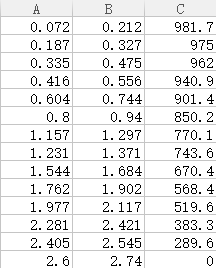
\includegraphics[width=0.4\textwidth]{fig/figure4.png}
\caption{H1=23cm,C-N}
\end{figure}
\begin{figure}[h!]
\centering
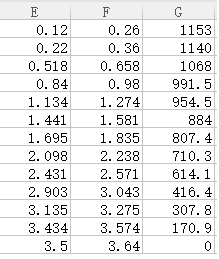
\includegraphics[width=0.5\textwidth]{fig/figure5.png}
\caption{H2=29cm,C-N}
\end{figure}

\begin{figure}[h!]
\centering
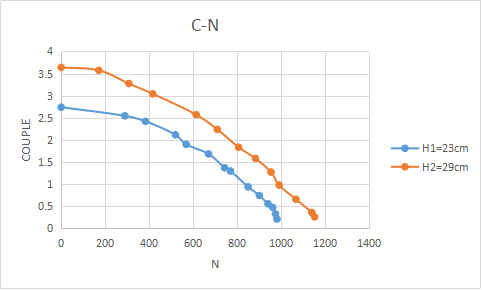
\includegraphics[width=1.0\textwidth]{fig/figure6.png}
\caption{couple en fonction de la vitesse de rotation}
\end{figure}

On voit que pour une hauteur de chute $Hm_1=23$, on trouve une gamme de vitesse supérieure à celle pour $Hm_2=29$, on remarque aussi que le coefficient directeur de la courbe rouge est moins important que celui de la courbe bleue, ceci est du au fait que le couple impacte plus la vitesse pour $Hm_2=29$.\\
\\
\section{P-N}

\begin{figure}[h!]
\centering
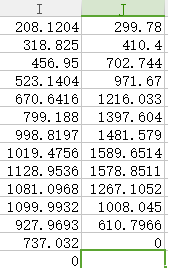
\includegraphics[width=0.4\textwidth]{fig/figure7.png}
\caption{P pour H1 et H2}
\end{figure}

\begin{figure}[h!]
\centering
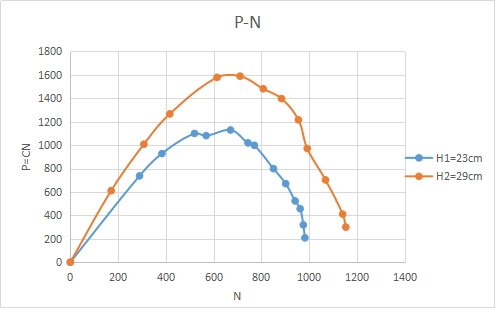
\includegraphics[width=1.0\textwidth]{fig/figure8.png}
\caption{P-N}
\end{figure}
Sur ce graphique, on voit que la puissance a tendance à décroître pour une grande vitesse de rotation.\\

On voit que le maximum de puissance est deux fois plus grand pour $Hm_1$ que pour $Hm_2$ mais le coefficient directeur de la courbe rouge est plus petit que celui de la courbe droite, ceci nous indique que la puissance décroît moins rapidement pour de petites hauteurs de chute, mais que la valeur de celle-ci reste supérieure pour de grandes hauteurs de chute.\\

\section{W-N}

\begin{figure}[h!]
\centering
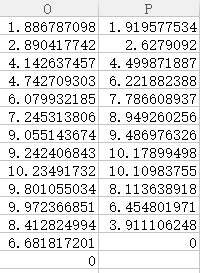
\includegraphics[width=0.4\textwidth]{fig/figure9.png}
\caption{$\omega$ coordonne}
\end{figure}\begin{figure}[h!]
\centering
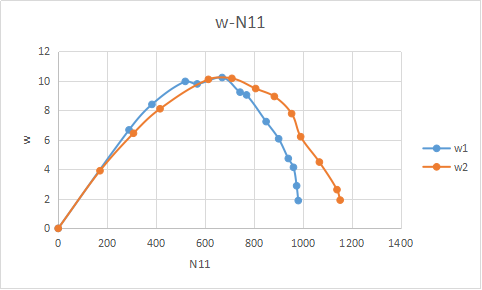
\includegraphics[width=1.0\textwidth]{fig/figure10.png}
\caption{$\omega$-$N_{11}$}
\end{figure}
Sur ce graphique, on voit que les deux courbes sont pratiquement confondues comme on s'y attendais, on peut faire l'hypothèse que le décalage entre les deux vient des erreurs de lecture pendant les différentes étapes expérimentales, mais aussi du fait qu'on ait pris des valeurs moyennes pour le couple et que le couple n'est pas parfait au niveau du contact avec l'arbre de la turbine.En effet, pendant la manipulation et le relevé des valeurs, à partir d'un certain couple, la machine subissait un emballement et la vitesse de rotation tendait rapidement vers 0 pendant que la valeur du couple tendait vers de très grandes valeurs.\\
\section{$\eta$-N}
\begin{figure}[h!]
\centering
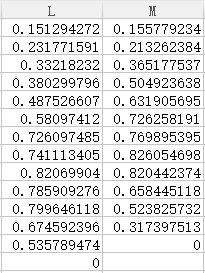
\includegraphics[width=0.4\textwidth]{fig/figure11.png}
\caption{$\eta$ coordonne}
\end{figure}\begin{figure}[h!]
\centering
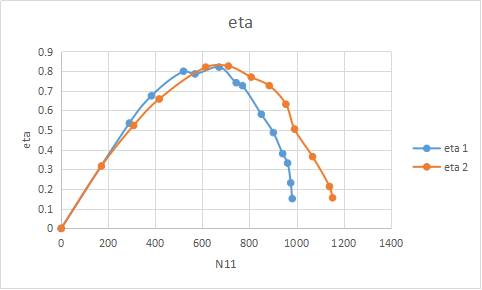
\includegraphics[width=0.9\textwidth]{fig/figure12.png}
\caption{$\eta$-$N_{11}$}
\end{figure}
Le but du dernier graphique est de comparer les rendements pour deux hauteurs de chute en fonction d'une vitesse de rotation adimensionnée, on voit que les deux courbes sont pratiquement confondues



\section{Reynolds nombre}
On calcul reynolds  nombre , on utilise la relation d'energie cinetique du jet à la sortie de l'injecteur :
$$V=\sqrt{2(gH_m-\frac{\triangle P}{P})}$$
$$L=\frac{d}{D}$$
$$Re=\frac{VL}{\nu}$$

apres applique numerique , on trouve $Re1 \simeq 98000 $,$ Re2 \simeq 86000$

on a les deux reynolds nombre plus grande que 4000 , et on dit que on a un écoulement turbulent dans mon etude .

\chapter{Conclusion}

1. Je fait cette TP tout seul , pour moi il est un peu difficile .\\

2. Repondre la question à la fin de TP : quand l'hauteur est 40m , la vitess de rotation ne augement pas . par ce-que la dbit est deja maximal .\\

3.Il y a une petite error dans la CR , l'unité est metre pour $H_1$ et $ H_2$.\\

4.Pour un meilleur etude de turbine , on prefere grande Reynolds nombre .

\end{document}
\grid